\documentclass[tikz,border=5mm]{standalone}
\usepackage{tikz}
\usetikzlibrary{shapes,arrows,positioning}
\usepackage{xcolor} % Ensure xcolor is loaded for colors

% Define colors
\definecolor{UFJFWine}{HTML}{7A0026}
\definecolor{UFJFLightGray}{HTML}{E6E6E6}
\definecolor{UFJFBlack}{HTML}{000000}

% New color scheme
\definecolor{WineLight}{HTML}{E8D5D8}  % Vinho claro para nodes
\definecolor{WineDark}{HTML}{5C001A}    % Vinho escuro para contorno/texto
\definecolor{BlueLight}{HTML}{D6E3F7}    % Azul claro para tópico
\definecolor{BlueDark}{HTML}{1E3A8A}    % Azul escuro para contorno/texto
\definecolor{GreenLight}{HTML}{D1FAE5}  % Verde claro para serviço
\definecolor{GreenDark}{HTML}{065F46}   % Verde escuro para contorno/texto
\definecolor{OrangeLight}{HTML}{FED7AA} % Laranja claro para ação
\definecolor{OrangeDark}{HTML}{9A3412}  % Laranja escuro para contorno/texto
\definecolor{GrayLight}{HTML}{F3F4F6}  % Cinza claro para parâmetros
\definecolor{GrayDark}{HTML}{374151}   % Cinza escuro para contorno/texto

\begin{document}
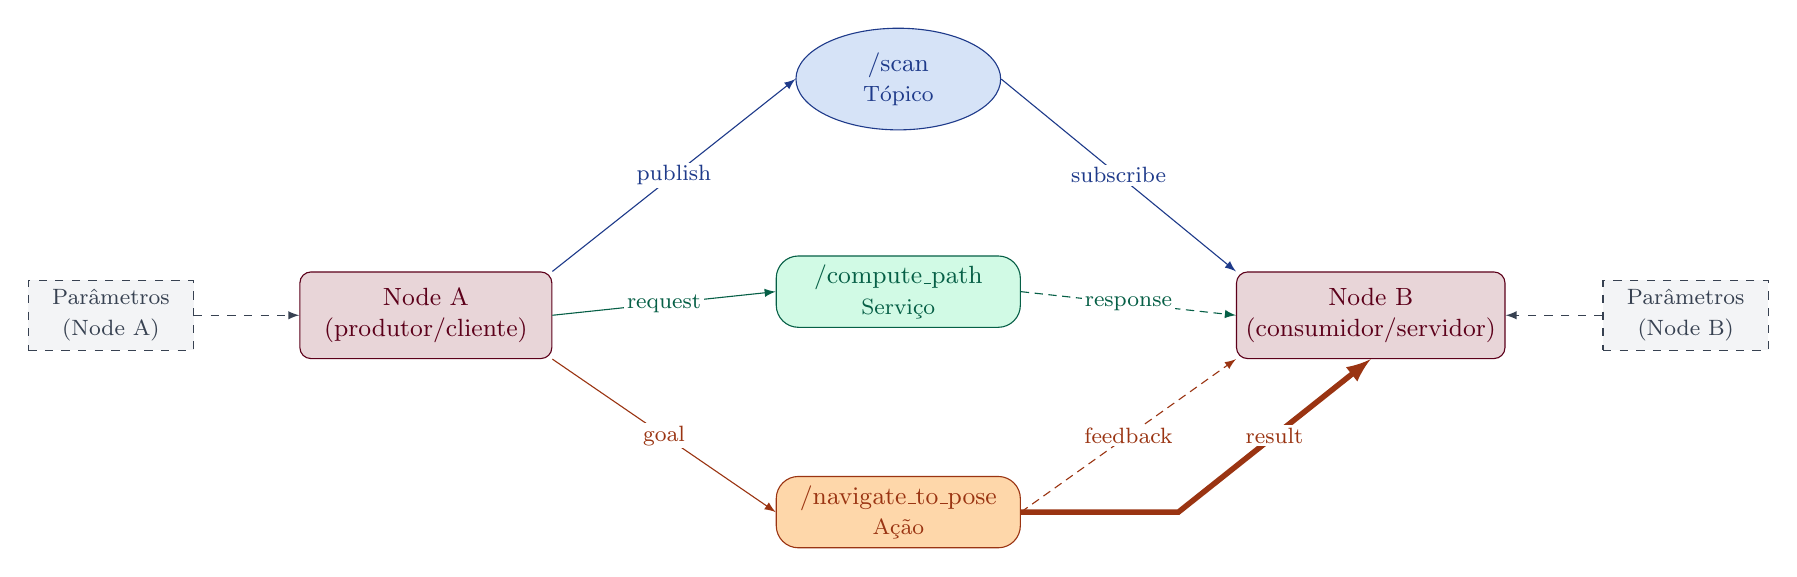
\begin{tikzpicture}[
  >=latex,
  font=\small,
  node/.style={draw=WineDark, fill=WineLight, rounded corners, align=center, minimum width=3.2cm, minimum height=1.1cm, text=WineDark},
  topic/.style={draw=BlueDark, fill=BlueLight, ellipse, align=center, minimum width=2.6cm, minimum height=1cm, text=BlueDark},
  iface/.style={draw=GreenDark, fill=GreenLight, rounded corners=8pt, align=center, minimum width=3.1cm, minimum height=0.9cm, text=GreenDark},
  action/.style={draw=OrangeDark, fill=OrangeLight, rounded corners=8pt, align=center, minimum width=3.1cm, minimum height=0.9cm, text=OrangeDark},
  param/.style={draw=GrayDark, fill=GrayLight, align=center, minimum width=2.1cm, minimum height=0.8cm, dashed, text=GrayDark},
  lbl/.style={midway, fill=white, inner sep=1pt}
]

% Nodes
\node[node] (A) at (0,0) {Node A\\(produtor/cliente)};
\node[node] (B) at (12,0) {Node B\\(consumidor/servidor)};

% Topic (pub/sub) - AZUL
\node[topic] (T) at (6,3) {/scan\\\footnotesize Tópico};
\draw[BlueDark,->] (A.north east) -- node[lbl,text=BlueDark]{\footnotesize publish} (T.west);
\draw[BlueDark,->] (T.east) -- node[lbl,text=BlueDark]{\footnotesize subscribe} (B.north west);

% Service (req/resp) - VERDE
\node[iface] (S) at (6,0.3) {/compute\_path\\\footnotesize Serviço};
\draw[GreenDark,->] (A.east) -- node[lbl,text=GreenDark]{\footnotesize request} (S.west);
\draw[GreenDark,densely dashed,->] (S.east) -- node[lbl,text=GreenDark]{\footnotesize response} (B.west);

% Action (goal/feedback/result) - LARANJA
\node[action] (Act) at (6,-2.5) {/navigate\_to\_pose\\\footnotesize Ação};
\draw[OrangeDark,->] (A.south east) -- node[lbl,text=OrangeDark]{\footnotesize goal} (Act.west);
\draw[OrangeDark,densely dashed,->] (Act.east) -- node[lbl,text=OrangeDark]{\footnotesize feedback} (B.south west);

% Result with detour - goes horizontally first, then up
\draw[OrangeDark,line width=2pt,->] (Act.east) -- ++(2,0) -- node[lbl,text=OrangeDark]{\footnotesize result} (B.south);

% Parameters (alinhados horizontalmente com os nodes) - CINZA
\node[param] (PA) at (-4,0) {\footnotesize Parâmetros\\ \footnotesize (Node A)};
\node[param] (PB) at (16,0) {\footnotesize Parâmetros\\ \footnotesize (Node B)};
\draw[GrayDark,dashed,->] (PA.east) -- (A.west);
\draw[GrayDark,dashed,->] (PB.west) -- (B.east);

\end{tikzpicture}
\end{document}